\subsubsection{KD-træer}
\label{sec:kdtree}

Et K-dimensionelt træ (KD-træ), er en abstrakt datastruktur som bl.a.\ andvendes til opdeling af 'rum'. Et KD-træ er repræsenteret som et binært træ, dvs.\ at
hver gren i træet har yderligere to grene indtil bladene nåes (se figur \ref{fig:binary-tree}) herunder. 

\begin{figure}[H]
  \centering
  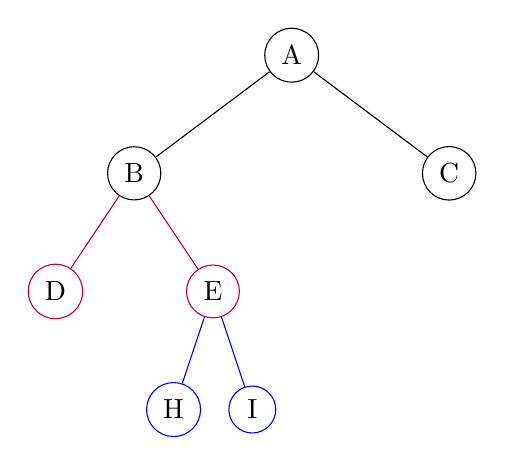
\begin{tikzpicture}[
    level 1/.style={sibling distance=40mm},
    level 2/.style={sibling distance=20mm},
    level 3/.style={sibling distance=10mm},
    every node/.style={draw,circle},
    arrow/.style={edge from parent/.style={draw,-latex}}
  ]
  \node {A}
    child[draw=black] { node{B}
      child[draw=purple] { node{D} }
      child[draw=purple] { node{E}
          child[draw=blue] {node{H}}
          child[draw=blue] {node{I}}
      }
    }
    child[draw=black] { node{C} }
  ;
  \end{tikzpicture}
  \caption{Binært træ}
  \label{fig:binary-tree}
\end{figure}

Med et KD-træ opdeles et rum efter værdier, højere eller lavere end et taktisk udvalgt delingspunkt (se figur \ref{fig:kd-tree-itteration}),
således at alle værdier i en gren, enten er højere eller lavere end den gren de udspringer fra. Denne  opdeling fortsætter indtil værdierne i en gren er trivielle at behandle, herved kaldes en sådan gren for et blad.

\begin{figure}[H]
  \begin{subfigure}{0.31\textwidth}
    % \centering
    \begin{tikzpicture}[width=\linewidth, scale=0.9]
      \coordinate (lowlow) at (0,0);
      \coordinate (lowhigh) at (0,5);
      \coordinate (highlow) at (5,0);
      \coordinate (highhigh) at (5,5);

      \coordinate (A1) at (0.4,0);
      \coordinate (A2) at (0,1);
      \coordinate (A3) at (2,0.3);

      \coordinate (B1) at (0.4,5);
      \coordinate (B2) at (2,4);
      \coordinate (B3) at (3,4.3);

      \coordinate (C1) at (5,3.6);
      \coordinate (C2) at (4,3);
      \coordinate (C3) at (4,1.3);

      \coordinate (D1) at (2,3.6);
      \coordinate (D2) at (0.6,3);
      \coordinate (D3) at (1.5,1.3);

      \path[fill=gray!10, draw=black!40] (lowlow) -- (lowhigh) -- (highhigh) -- (highlow) -- (lowlow);
      
      \path[fill=blue!50, draw=blue!20] (A1) -- (A2) -- (A3) -- (A1);
      \path[fill=blue!50, draw=blue!20] (B1) -- (B2) -- (B3) -- (B1);
      \path[fill=blue!50, draw=blue!20] (C1) -- (C2) -- (C3) -- (C1);
      \path[fill=blue!50, draw=blue!20] (D1) -- (D2) -- (D3) -- (D1);
    
      \node [above] at (2.5, 2.25) {$A$};

    \end{tikzpicture}
    \caption{Rod}
    \label{fig:kd-tree-initial}
  \end{subfigure}
  \hspace*{\fill} % separation between the subfigures
  \begin{subfigure}{0.31\textwidth}
    % \centering
    \begin{tikzpicture}[width=\linewidth, scale=0.9]
      \coordinate (lowlow) at (0,0);
      \coordinate (lowhigh) at (0,5);
      \coordinate (highlow) at (5,0);
      \coordinate (highhigh) at (5,5);

      \coordinate (A1) at (0.4,0);
      \coordinate (A2) at (0,1);
      \coordinate (A3) at (2,0.3);

      \coordinate (B1) at (0.4,5);
      \coordinate (B2) at (2,4);
      \coordinate (B3) at (3,4.3);

      \coordinate (C1) at (5,3.6);
      \coordinate (C2) at (4,3);
      \coordinate (C3) at (4,1.3);

      \coordinate (D1) at (2,3.6);
      \coordinate (D2) at (0.6,3);
      \coordinate (D3) at (1.5,1.3);

      \path[fill=gray!10, draw=black!40] (lowlow) -- (lowhigh) -- (highhigh) -- (highlow) -- (lowlow);
      
      \path[fill=blue!50, draw=blue!20] (A1) -- (A2) -- (A3) -- (A1);
      \path[fill=blue!50, draw=blue!20] (B1) -- (B2) -- (B3) -- (B1);
      \path[fill=blue!50, draw=blue!20] (C1) -- (C2) -- (C3) -- (C1);
      \path[fill=blue!50, draw=blue!20] (D1) -- (D2) -- (D3) -- (D1);
      
      \draw [black, thick] (3, 5) -- (3, 0);

      \node [above] at (1.5, 2.25) {$B$};
      \node [above] at (4, 2.25) {$C$};
    \end{tikzpicture}
  \caption{Første itteration}
  \label{fig:kd-tree-itteration}
  \end{subfigure}
  \hspace*{\fill} % separation between the subfigures
  \begin{subfigure}{0.31\textwidth}
    % \centering
    \begin{tikzpicture}[width=\linewidth, scale=0.9]
      \coordinate (lowlow) at (0,0);
      \coordinate (lowhigh) at (0,5);
      \coordinate (highlow) at (5,0);
      \coordinate (highhigh) at (5,5);

      \coordinate (A1) at (0.4,0);
      \coordinate (A2) at (0,1);
      \coordinate (A3) at (2,0.3);

      \coordinate (B1) at (0.4,5);
      \coordinate (B2) at (2,4);
      \coordinate (B3) at (3,4.3);

      \coordinate (C1) at (5,3.6);
      \coordinate (C2) at (4,3);
      \coordinate (C3) at (4,1.3);

      \coordinate (D1) at (2,3.6);
      \coordinate (D2) at (0.6,3);
      \coordinate (D3) at (1.5,1.3);

      \path[fill=gray!10, draw=black!40] (lowlow) -- (lowhigh) -- (highhigh) -- (highlow) -- (lowlow);
      
      \path[fill=blue!50, draw=blue!20] (A1) -- (A2) -- (A3) -- (A1);
      \path[fill=blue!50, draw=blue!20] (B1) -- (B2) -- (B3) -- (B1);
      \path[fill=blue!50, draw=blue!20] (C1) -- (C2) -- (C3) -- (C1);
      \path[fill=blue!50, draw=blue!20] (D1) -- (D2) -- (D3) -- (D1);
      
      \draw [black, thick] (3, 5) -- (3, 0);
      \draw [purple, thick] (0, 3.6) -- (3,  3.6);
      \draw [blue, thick] (0,  1) -- (3,   1);
      
      \node [above] at (4, 2.25) {$C$};
      \node [above] at (1.5, 4.05) {$D$};
      \node [above] at (1.5, 2.05) {$F$};
      \node [above] at (1.5, 0.25) {$G$};
    \end{tikzpicture}
  \caption{Færdigbygget KD-træ}
  \label{fig:kd-tree-finished}
  \end{subfigure}
  \caption{KD-træ}
  \label{fig:kd-tree-example}
\end{figure}

Et eksempel på opbygningen af et KD-træ ses i figur \ref{fig:kd-tree-example}. Et KD-træ starter med roden (figur \ref{fig:kd-tree-initial}), som omkranser hele data-mængden. Herefter opdeles alle non-trivielle grene i yderligere to grene (figur \ref{fig:kd-tree-itteration}), dette gentages indtil alle grene/blade er et simpelt tilfælde (figur \ref{fig:kd-tree-finished}).